\documentclass[11pt,a4]{article}
\usepackage[utf8]{inputenc}
\usepackage[catalan]{babel}

\usepackage{geometry} %% Marges
\geometry{
    a4paper,
    left=25mm,
    right=25mm,
    top=25mm,
    bottom=25mm,
}

%% Simbols, AMS, etc

\usepackage{amsmath}
\usepackage{amssymb}
\usepackage{amsthm}
\usepackage{esint}
\usepackage{braket}

%% Titols, seccions, etc

\usepackage{titling} %% Permet cridar thetitle, etc

%% Enumeracions, hipervincles

\usepackage{enumerate}
\usepackage{hyperref}

%% Text Lipsum
\usepackage{lipsum}

%% Colors i codi

\usepackage[dvipsnames]{xcolor}
\usepackage{color}
\definecolor{blueblack}{rgb}{0,0,0.5}
\hypersetup{
    colorlinks,
    citecolor=black,
    filecolor=black,
    linkcolor=blueblack,
    urlcolor=black
}
\usepackage{listings}
\lstset{aboveskip=15pt,belowskip=15pt}
\renewcommand{\lstlistingname}{Codi} % Listing -> Codi
\renewcommand{\ttdefault}{cmtt} % Bold tt font

%% Definicio d'alguns colors per al codi lstlisting

\definecolor{codegreen}{rgb}{0,0.6,0}
\definecolor{codegray}{rgb}{0.5,0.5,0.5}
\definecolor{codepurple}{rgb}{0.58,0,0.82}
\definecolor{backcolour}{rgb}{0.95,0.95,0.92}
 
\lstdefinestyle{mystyle}{
    backgroundcolor=\color{backcolour},   
    commentstyle=\color{codegreen},
    keywordstyle=\bfseries\color{magenta},
    numberstyle=\tiny\color{codegray},
    stringstyle=\color{codepurple},
    basicstyle=\footnotesize\ttfamily,
    breakatwhitespace=false,         
    breaklines=true,                 
    captionpos=b,                    
    keepspaces=true,                 
    numbers=left,                    
    numbersep=5pt,                  
    showspaces=false,                
    showstringspaces=false,
    showtabs=false,                  
    tabsize=2
}
\lstset{style=mystyle} % Escollim mystyle com a estil per defecte

%% Teoremes i estil

\makeatletter
\newtheoremstyle{thmstyle}
  {5pt}% space before
  {5pt}% space after
  {\addtolength{\@totalleftmargin}{3.5em}
   \addtolength{\linewidth}{-3.5em}
   \parshape 1 2em \linewidth \bfseries}% body font
  {0pt}% indent
  {\bfseries}% header font
  {.}% punctuation
  {.5em}% after theorem header
  {}% header specification (empty for default)
\makeatother

\numberwithin{equation}{section}
  \theoremstyle{thmstyle}
  \newtheorem{Definition}{Definició}
  \theoremstyle{thmstyle}
  \newtheorem*{Theorem}{Teorema}
  \theoremstyle{thmstyle}
  \newtheorem{Proposition}{Proposició}
  \theoremstyle{thmstyle}
  \newtheorem{Corollary}{Corol·lari}
  \theoremstyle{thmstyle}
  \newtheorem{Lemma}{Lema}
  \theoremstyle{thmstyle}
  \newtheorem{question}{Qüestió}
  \theoremstyle{thmstyle}
  \newtheorem{activity}{Activitat}
  
%% Comandes

\newcommand{\bs}{\mathbf}
\newcommand{\mc}{\mathcal}
\newcommand{\mb}{\mathbb}
\newcommand{\dif}{\mathrm{d}}
\newcommand{\Fourier}{\mc{F}}
\newcommand{\salto}{\vspace{12pt} \noindent}
\newcommand{\sinc}{\mathrm{sinc}\,}
\newcommand{\IIR}{\mathrm{IIR}}
\renewcommand{\ss}{\scriptstyle}

%% PGF i TIKZ

\usepackage{tikz,pgfplots}
\pgfplotsset{compat=1.5, width=15cm, height=10cm, scale only axis}

%% Encapçalament i peu de pàgina

\usepackage{fancyhdr}
\pagestyle{fancy}
\fancyhf{}
\fancyhead[LE,RO]{\thetitle}
\fancyhead[RE,LO]{\theauthor}
\fancyfoot[CE,CO]{}
\fancyfoot[LE,RO]{\thepage}

\title{Teoria del Senyal. Pràctica 2 de laboratori}
\author{Eric Guisado, Raúl Alonso}

\begin{document}

%% PGF set
\pgfplotsset{
    standard/.style={%Axis format configuration
        axis x line=middle,
        axis y line=middle,
        enlarge x limits=0.15,
        enlarge y limits=0.15,
        every axis x label/.style={at={(current axis.right of origin)},anchor=north west},
        every axis y label/.style={at={(current axis.above origin)},anchor=north east},
        every axis plot post/.style={mark options={fill=white}}
        }
    }

\thispagestyle{empty}

\noindent
{\bf \LARGE \thetitle}

\noindent
\rule{\textwidth}{1pt}

\vspace{15pt}

\noindent
{\Large \theauthor}
\vspace{15pt}

\noindent
{\large Divendres 30 de setembre de 2016}
\vspace{15pt}

\tableofcontents

\section{Estudi previ}
\begin{question}
Si el senyal d’entrada x[n] té longitud $L_x$, indicar quina seria la longitud $L_y$ del senyal resultat del filtratge y[n] en funció de $L$ i $L_x$. Indicar quantes multiplicacions s’han de fer per poder calcular les $L_y$ mostres del senyal de sortida mitjançant l’aplicació directa de l’equació de convolució suposant que $L_x > L$. Expressar aquest número de multiplicacions en funció de $L$ i $L_x$. Calcular també el número de multiplicacions per mostra d’entrada (és a dir, el quocient entre el número total de multiplicacions necessàries i el número de mostres d’entrada $L_x$).
\end{question}

El senyal de sortida y[n] es calcula com 

$$
y[n]=\lbrace x\ast h\rbrace[n]=\sum_{j=0}^{L-1} h[j]x[n-j]
$$

Suposem que el senyal $x[n]$ comença a $n=k$ i acaba a $n=k+L_x-1$. Els termes de la sortida $y[n]$ seran aquells per als quals hi ha algun $j\in\lbrace 0, 1, ..., L-1\rbrace$ tal que $n-j\in \lbrace k, k+1, ..., k+L_x-1\rbrace$, és a dir, $k\leqslant n-j \leqslant k+L_x-1 \Longleftrightarrow k+j\leqslant n \leqslant k+L_x-1+j$. Per tant, els termes de la sortida seran aquells amb $k\leqslant n \leq k+L_x+L-2$. Així doncs, la sortida té longitud $L+L_x-1$.

Observem que podem escriure, per a $k\leqslant n \leq k+L_x+L-2$:

$$
y[n]=\lbrace x\ast h\rbrace[n]=\sum_{j=\max{\lbrace 0, n-k-L_x+1\rbrace}}^{\min{\lbrace L-1,n-k\rbrace}} h[j]x[n-j] = 
$$
$$
\begin{cases}
\sum_{j=0}^{n-k} h[j]x[n-j]  & \text{si $k \leqslant n \leqslant k + L - 1$} \\
\sum_{j=0}^{L-1} h[j]x[n-j]  & \text{si $k+L-1 < n < k + L_x - 1$} \\
\sum_{j=n-k-L_x+1}^{L-1} h[j]x[n-j]  & \text{si $k + L_x - 1 \leqslant n \leqslant k + L + L_x - 2$}
\end{cases}
$$

Així, es dedueix que el nombre de multiplicacions que cal fer en aplicar directament l'equació de convolució és:
$$
2\sum_{i=1}^{L} i + L(L_x - L - 1) = L(L+1)+L(L_x-L-1)=LL_x
$$

El nombre de multiplicacions per mostra d'entrada és $\frac{LL_x}{L_x}=L$.

\begin{question}
Respon a les següents preguntes:
\begin{enumerate}[a)]
\item Relacionar el número de blocs $P$ ($i=0,...,P-1$) amb $L_x$ i $M$.
\item Quin és el valor màxim de $M$ (donat el número de punts totals $N$ de cada bloc $x_i[n]$) per tal que la convolució circular en (1) coincideixi amb la convolució lineal en (2)?
Expressar aquest valor màxim de $M$ en funció de $N$ i $L$.
\end{enumerate}
\end{question}

Cada trama ve donada per
$$
x_i[n] =
\begin{cases}
x[n + iM] & i = 0,\ldots,M - 1 \\
0         & i = M, \ldots, N - 1
\end{cases},
$$
i cadascuna d'aquestes es correspon amb el segment de $x$ que va des de $x[iM]$ fins a $x[i(M + 1) - 1]$, afegint-hi zeros al darrere fins que aquesta trama tingui mida $N$. Si volem que aquestes trames recorrin tot el senyal $x$, i que no n'hi hagi cap més que les necessàries, cal que el darrer $i$ que agafem contingui el darrer element de $x$, és a dir, per a $i = P - 1$ hi ha d'haver algun $n$, amb $0 \leq n \leq M - 1$, tal que $L_x - 1 = (P-1)M + n$. Cal, doncs, $(P-1)M\leqslant L_x - 1 \leqslant PM - 1$. Per tant, necessitem
$$
\frac{L_x}{M}\leqslant P \leqslant \frac{L_x + M - 1}{M}.
$$
Així doncs, $P$ ha de ser $P = \big\lceil\frac{L_x}{M}\big\rceil$.

Per tal que la convolució circular coincideixi amb la convolució lineal s'ha de verificar, per a $n\in\lbrace 0, 1, \cdots, N-1 \rbrace$:

$$
\sum_{j=0}^{L-1} h[j]x_i[n-j] = \sum_{j=0}^{L-1} h[j]\sum_{r=-\infty}^{\infty}x_i[n-j-rN]
$$

Per garantir-ho, imposem que, per a $r\neq 0$, $n\in\lbrace 0, 1, \cdots, N-1 \rbrace$, $j\in\lbrace 0, 1, \cdots, L-1 \rbrace$, $n-j-rN\not\in \lbrace 0, 1, \cdots, M-1 \rbrace$.

Per a $r>0$, veiem que sempre es té $n-j-rN<0$. En efecte, el màxim valor d'aquesta expressió es dóna amb $r = 1$, $j=0$, $n=N-1$, i és $-1$.

Per a $r>0$, veiem que sempre es té $n-j-rN\geqslant M$. En aquest cas, el mínim valor d'aquesta expressió es dóna amb $r = -1$, $j=L-1$ i $n=0$. S'ha de satisfer, doncs, $N-L+1\geqslant M$. Per tant, el valor màxim de $M$ és $N-L+1$.

(Altrament, la convolució circular és la suma dels senyals que s'obtenen aplicant un retard de $rN$, amb $r\in\mathbb{Z}$. Per evitar encavallaments, la longitud de la convolució lineal ha de ser menor que $N$. Per tant, $L+M-1\leqslant N$.)

\begin{question}
Calcular el número de multiplicacions reals associat a aquest mètode per mostra d’entrada. Per això, considerar que es fa ús de l’algorisme FFT suposant que el número de punts de la DFT és una potència de 2, és a dir, $N=2^\nu$ (en aquest cas, el número de multiplicacions complexes tant de la DFT com de la IDFT és de $N\log_2 N$ multiplicacions complexes). Considerar també que el valor de $M$ és el valor màxim calculat
a la qüestió 2.2. Per a calcular el número de multiplicacions per mostra d’entrada s’ha de calcular quantes multiplicacions són necessàries per a processar cada bloc i dividir aquest número per $M$, és a dir, pel número de mostres d’entrada que es processen a cada bloc. Expressar el resultat en funció de $L$ i $N$.
\end{question}

Per trobar la DFT d'un bloc i, després d'obtenir el producte $X_i[k]H[k]$, trobar-ne la transformada inversa calen $2N\log_2 N$ multiplicacions complexes. El producte $X_i[k]H[k]$ requereix $N$ multiplicacions complexes. El nombre d'operacions per mostra d'entrada és, doncs:

$$
\frac{2N\log_2 N + N}{M} = \frac{2N\log_2 N + N}{N-L+1} = \frac{2\log_2 N + 1}{1-\frac{L-1}{N}}
$$

\begin{question}
Escriure una funció en MATLAB {\tt function yb = cc(xb,H)} que calculi la convolució circular de {\tt N} punts de {\tt xb} amb {\tt h}. Suposi que el vector d'entrada {\tt H} ja conté la DFT de {\tt N} punts de {\tt h}. El càlcul del resultat, que s'ha de retornar mitjançant el vector {\tt yb}, s'ha de calcular com la IDFT de {\tt N} punts:
$$
yb[n] = IDFT_N [Xb[k]H[k]].
$$
Creï la funció ``process''. Aquest funció tindrà la següent capçalera: {\tt function y = process(x,h,N)}.
\end{question}

Les dues funcions es troben en els fitxers {\tt cc.m} i {\tt process.m}, respectivament.

\begin{lstlisting}[language=MATLAB]
function[yb] = cc(xb,H)
N = length(H);
X = fft(xb,N);
Y = X.*H;
yb = ifft(Y,N);
end
\end{lstlisting}

\begin{lstlisting}[language=MATLAB]
function[y] = process(x,h,N)
L = length(h);
Lx = length(x);
H = fft(h,N);
M = N - L + 1;
P = floor(Lx/M);
y=zeros(1, L+Lx-1);
for i = 0 : P - 1
    xb = x(i*M+1:(i+1)*M);
    yb = cc(xb,H);
    y(i*M+1:i*M+N) = y(i*M+1:i*M+N) + yb;
end
xb = x(P*M+1:Lx);
yb = cc(xb,H);
y(P*M+1:P+Lx-1) = y(P*M+1:P+Lx-1) + yb;
end
\end{lstlisting}

\begin{question}
Quina és l'expressió matemàtica corresponent a la DFT de $N$ punts d'un senyal sinusoïdal de pulsació discreta $\Omega_0=2\pi\frac{k_0}{N}$ (essent $k_0$ un número enter)?
\end{question}

En primer lloc, observem que podem suposar $k_0\in\lbrace 0,1,\cdots,N-1\rbrace$, ja que, si $k_0=qN+r$, amb $q\in\mathbb{Z}$ i $r\in\lbrace 0,1,\cdots,N-1\rbrace$, llavors:

$$
\sin(2\pi\frac{k_0}{N}n) = \sin(2\pi qn + 2\pi\frac{r}{N}n) = \sin(2\pi\frac{r}{N}n) \quad \forall n\in\mathbb{Z}.
$$

La DFT de $N$ punts del senyal $x[n]=\sin(2\pi\frac{k_0}{N}n)$, $n=0,1,\cdots, N-1$ ve donada per:

$$X[k] = \sum_{n=0}^{N-1}\sin(2\pi\frac{k_0}{N}n)e^{-j2\pi\frac{k}{N}n} = \sum_{n=0}^{N-1}\Big(\frac{e^{j2\pi\frac{k_0}{N}n}-e^{-j2\pi\frac{k_0}{N}n}}{2j}\Big)e^{-j2\pi\frac{k}{N}n}=
$$
$$
=\frac{1}{2j}\Big(\sum_{n=0}^{N-1}e^{-j2\pi\frac{(k-k_0)}{N}n}-\sum_{n=0}^{N-1}e^{-j2\pi\frac{(k+k_0)}{N}n}\Big)=
$$
$$
\begin{cases}
0                 & \text{si $k=k_0=N-k_0$ (només pot passar si $k_0 = N/2$)} \\
-j\frac{N}{2}     & \text{si $k=k_0\neq N-k_0$} \\
+j\frac{N}{2}     & \text{si $k=N-k_0\neq k_0$} \\
0                 & \text{altrament}
\end{cases}
$$
En efecte, per a $k\in\lbrace 0,1,\cdots,N-1\rbrace$, $k\neq k_0$, $e^{-j2\pi\frac{(k-k_0)}{N}}\neq 1$, i per tant,
$$
\sum_{n=0}^{N-1}e^{-j2\pi\frac{(k-k_0)}{N}n}=\frac{1-e^{-j2\pi\frac{(k-k_0)}{N}N}}{1-e^{-j2\pi\frac{(k-k_0)}{N}}} = 0,
$$
i, anàlogament, si $k\in\lbrace 0,1,\cdots,N-1\rbrace$, $k\neq N-k_0$,
$$
\sum_{n=0}^{N-1}e^{-j2\pi\frac{(k+k_0)}{N}n}=\frac{1-e^{-j2\pi\frac{(k+k_0)}{N}N}}{1-e^{-j2\pi\frac{(k+k_0)}{N}}} = 0
$$

\begin{question}
Dibuixi la DFT d'aquest senyal sinusoïdal.
\end{question}

\begin{figure}[ht]
\centering
   \begin{tikzpicture}[scale = 0.9]
       \draw [->] (-0.8,0) -- (8,0);       
       \draw [->] (0,-0.8) -- (0,6.5);
       \node at (2,0) {$\ss |$};
       \node at (2,-0.4) {$\ss k_0$};
       \draw [thick] (2,0) -- (2,5);
       \node at (2,5) {\textbullet};
       \node at (2,5) [anchor=south]{$\angle = -\frac{\pi}{2}$};
       \node at (5.5,0) {$\ss |$};
       \node at (5.5,-0.4) {$\ss N-k_0$};
       \draw [thick] (5.5,0) -- (5.5,5);
       \node at (5.5,5) {\textbullet};
       \node at (5.5,5) [anchor=south]{$\angle = \frac{\pi}{2}$};
       \draw [dashed, thick] (0,5) -- (7.5,5);
       \node at (0,5) [anchor=east] {$\frac{N}{2}$};
       \node at (-0.3,-0.4) {$0$};
       \node at (7.5,0) {$\ss |$};
       \node at (7.5,-0.4) {$\ss N - 1$};
   \end{tikzpicture}
\end{figure}

\begin{question}
Expliqui qualitativament l’efecte d’aplicar “zero-padding” i una finestra no rectangular sobre la DFT.
\end{question}
El resultat d'aplicar zero-padding és que, com que el nombre de mostres de la DFT és més gran, tenim més informació sobre la transformada de Fourier contínua de la seqüència. En el cas del senyal sinusoïdal anterior, hi hauria més punts $X[k]$ diferents de zero.

Aplicar diferents tipus de finestres, si es fa adientment, ens pot permetre resaltar certs aspectes del senyal o reduir el soroll degut a l'enfinestrament.

\section{Activitat al laboratori}

\subsection{Part 0}

En aquest apartat comentarem breument el que férem al laboratori.

En primer lloc, connectàrem un dels generadors de senyals a l'oscil·loscopi i a l'analitzador de freqüències  i generàrem un senyal rectangular de freqüència ?. Per observar-lo a l'analitzador de freqüències haguérem d'ajustar la freqüència central i el rang de freqüències que volíem observar. 

Com sabem, al domini de la freqüència, en mòdul, un senyal rectangular periòdic de freqüència $\omega_0$ és una suma de deltes centrades als múltiples parells de la freqüència $\omega_0$ ($\omega = 2k\omega_0$) i d'àrea $\frac{4}{2k\omega_0}$, és a dir:

$$
\vert X(\omega)\vert = \sum_{k = -\infty}^{+\infty} \frac{4}{2k\omega_0}\delta(\omega-2k\omega_0)
$$

En canvi, l'espectre de freqüències que observàrem, a més dels pics corresponents a aquestes freqüències, presentava pics més petits als múltiples senars de $\omega_0$, i un cert soroll que s'estenia per tot el rang de freqüències, degut principalment a que el senyal generat no era un senyal rectangular periòdic perfecte (en particular, que el valor absolut del màxim del senyal rectangular no coincidís amb el del mínim explicaria l'aparició dels pics secundaris).

Tot seguit férem el mateix amb un senyal sinusoïdal. 

\subsection{Part 1}

\begin{activity}
Generi un vector aleatori $h$ de longitud $L=10^3$ mostres i un altre vector aleatori $x$ de longitud $L_x=10^7$. Per generar els vectors pot utilitzar la funció {\tt randn} de MATLAB. Mitjançant les instruccions {\tt tic} i {\tt toc} de MATLAB pot mesurar aproximadament el temps que passa entre l’execució de les dues instruccions. Compari la durada de l’execució de cada mètode per a diferents valors de $v$ on $N=2^v$ (essent $N$ una potència de 2 suficientment gran) i comprovi que els dos resultats de la convolució y1 i y2 són iguals.
\end{activity}

A la taula \ref{tb:temps} representem els diferents temps d'execució (aproximats) de la funció {\tt process} per a diferents valors de $v$ ($N = 2^v$). Ho representem gràficament a la figura \ref{fig:temps}. Tot i que els temps d'execució tinguin petits alts i baixos en la zona central de la gràfica, assumim que aquests provenen del fet que l'ordinador està realitzant altres processos paral·lelament que modifiquen el temps d'execució. Per tant, aquesta corba hauria de ser més semblant a una forma d'`U', i en el mig trobaríem el temps d'execució mínim, per a un valor òptim de $v$.

A la figura \ref{fig:teoric} hem representat el nombre d'operacions teòric de la funció {\tt process} en funció de $v$, segons la fórmula del nombre d'operacions que hem obtingut a la qüestió 2.3 de l'estudi previ:
$$
\text{nombre d'operacions} = \frac{2\log_2 N + 1}{1-\frac{L-1}{N}} =
\frac{2v + 1}{1-\frac{L-1}{2^v}}, \quad L = 10^3
$$

Podeu comprovar com les corbes de les figures \ref{fig:temps} i \ref{fig:teoric} són molt semblants.

\begin{table}
\centering
\begin{tabular}{|c|c|}
\hline
$v$       & temps de {\tt process} [s]  \\
11        & 1.068             \\
12        & 0.631             \\
13        & 0.517             \\
14        & 0.540             \\
15        & 0.466             \\
16        & 0.559             \\
17        & 0.599             \\
18        & 0.828             \\
19        & 0.907             \\
\hline
\end{tabular}
\caption{Taula dels diferents temps d'execució de la funció {\tt process} en funció de la potència $v$ de 2 ($N = 2^v$).}
\label{tb:temps}
\end{table}

\begin{figure}[h]
\centering
\begin{tikzpicture}[scale=0.7]
\begin{axis}[
  xlabel=$v$,
  ylabel=temps de {\tt process} (s)]
\addplot table [y=temps, x=v]{data.dat};
\addlegendentry{temps}
\end{axis}
\end{tikzpicture}
\caption{Representació gràfica dels valors de la taula \ref{tb:temps}.}
\label{fig:temps}
\end{figure}

\begin{figure}[h]
\centering
\begin{tikzpicture}[scale=0.7]
\begin{axis}[
  xlabel=$v$,
  ylabel=nombre d'operacions de {\tt process}]
\addplot [
    domain=11:19, 
    samples=100, 
    color=red,
    very thick,
]
{(2*x+1)/(1-(999/(2^x)))};
\addlegendentry{corba teòrica}
\end{axis}
\end{tikzpicture}
\caption{Representació del nombre d'operacions de {\tt process} en funció de $v$, amb $N = 2^v$.}
\label{fig:teoric}
\end{figure}

Hem obtingut els dos productes de convolució $y_1$ i $y_2$ amb les funcions {\tt conv} i {\tt process} respectivament. Hem pogut comprovar que els dos vectors resultants són (pràcticament) iguals, ja que l'error quadràtic, és a dir, la norma 2 del vector $k = y_1 - y_2$ és, per a $v=15$, $\epsilon = \Vert k \Vert_2 = 1.1684 \cdot 10^{-10}$.

\begin{activity}
Utilitzant la funció “load” de MATLAB, carregui el fitxer XX.mat. Després de carregar el fitxer, el senyal $x$ estarà disponible al workspace de MATLAB per a poder operar amb ell. Sabent que el senyal $x$ s’ha obtingut mitjançant un procés de mostreig prenent com a freqüència de mostreig $fs = 8 kHz$, porti a terme les següents activitats:
\begin{enumerate}[-]
\item Dibuixi el senyal $x$.
\item Quina és la duració del senyal $x$ en número de mostres i en segons?
\item Pot escoltar el so dels dos tons fent: wavplay(x,fs).
\item Obtingui la DFT de x (X[k]) i dibuixi el seu mòdul.
\item Mitjançant l’anàlisi del mòdul de la DFT de x, respongui a les següents qüestions:
\begin{enumerate}[$\circ$]
\item Trobi els índexs (valors de k) per a cadascun dels 4 pics de la DFT (pot utilitzar
la funció max de MATLAB).
\item Obtingui les freqüències digitals corresponents als dos pics detectats.
\item Quines són les freqüències analògiques (en Hz) corresponents a la freqüències
digitals anteriors?
\item Quina és la tecla corresponent al senyal x utilitzant la Figura 1?
\item Quina és l’amplitud dels pics de la DFT?
\item A partir del resultat anterior, calculi l’amplitud dels dos tons utilitzats en el
senyal x.
\end{enumerate}
\end{enumerate}
\end{activity}

Hem carregat el fitxer N1.MAT. El vector $x$ que ens donen, amb $1024$ mostres, és el resultat de mostrejar un senyal amb període de mostreig $T=\frac{1}{8000}\,s$. Per tant, la separació temporal entre mostres és $T$. La representació del senyal es pot veure a la figura \ref{fig:senyalx}.
\\

\begin{figure}
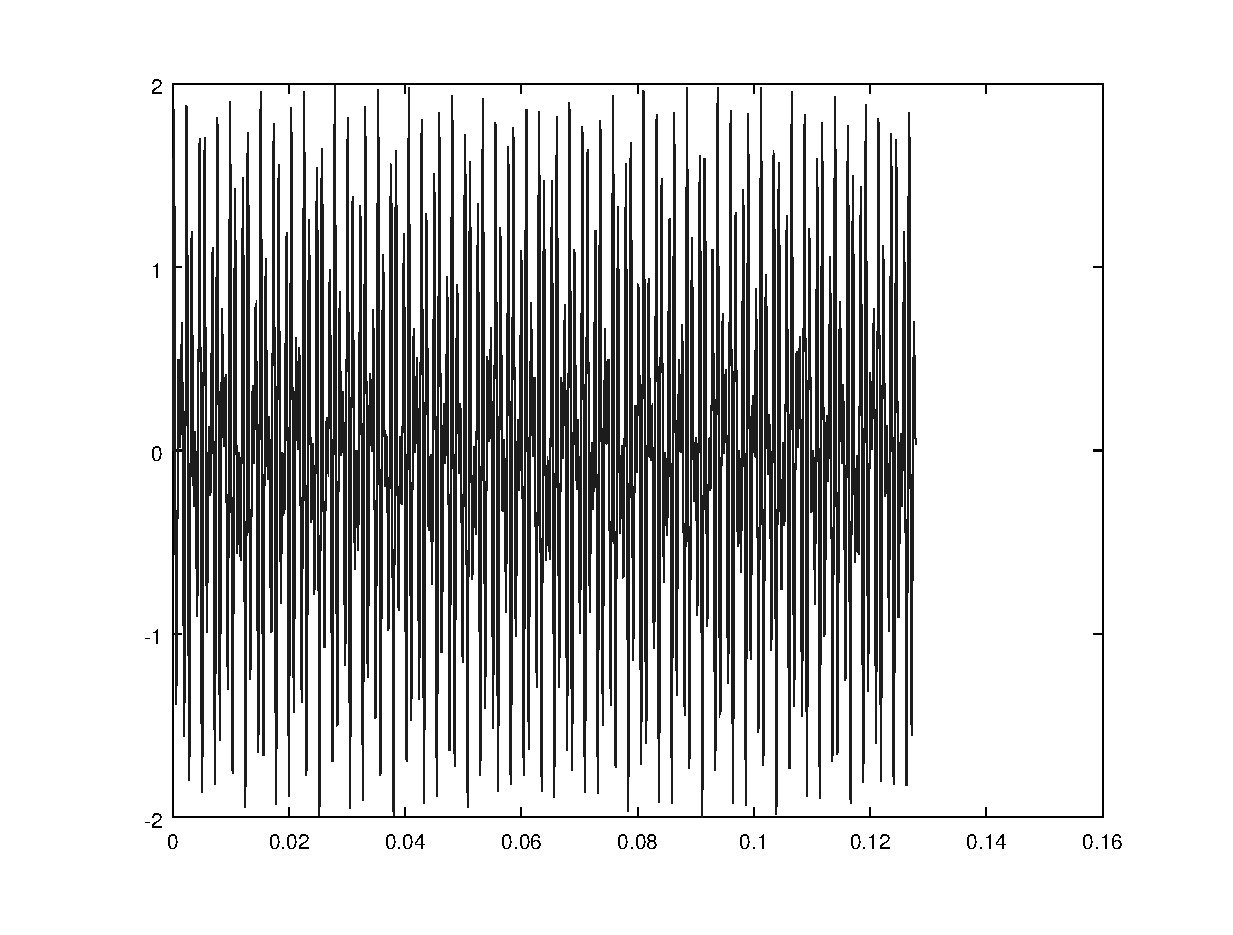
\includegraphics[scale=0.7]{senyalx.eps} 
\caption{Senyal $x$ al domini del temps.}
\label{fig:senyalx}
\end{figure}

La durada del senyal en mostres és $1024$. En temps, la seva durada és $\frac{1024}{8000}\,s=0,128\,s$.
\\

A la figura \ref{fig:moddft} podem observar la representació de la DFT de $8000$ punts de $x$, $X[k]$. Com podem veure, aquesta presenta quatre pics, que es troben a les posicions $k=941$ ($X[941] = 3,71-j511,46$, $\vert X[941]\vert=511,48$), $k=1336$ ($X[1336] = 2,88-j511,33$, $\vert X[1336]\vert=511,34$), $k=6664$ ($X[6664] = 3,71+j511,46$, $\vert X[6664]\vert=511,34$) i $7059$ ($X[7059] = 3,71+j511,46$, $\vert X[7059]\vert=511,48$). (Com que el senyal $x$ és real, $X[k] = X[8000-k]^\ast$, i, per tant, $\vert X[k]\vert = \vert X[8000-k]\vert$.)
\\

\begin{figure}
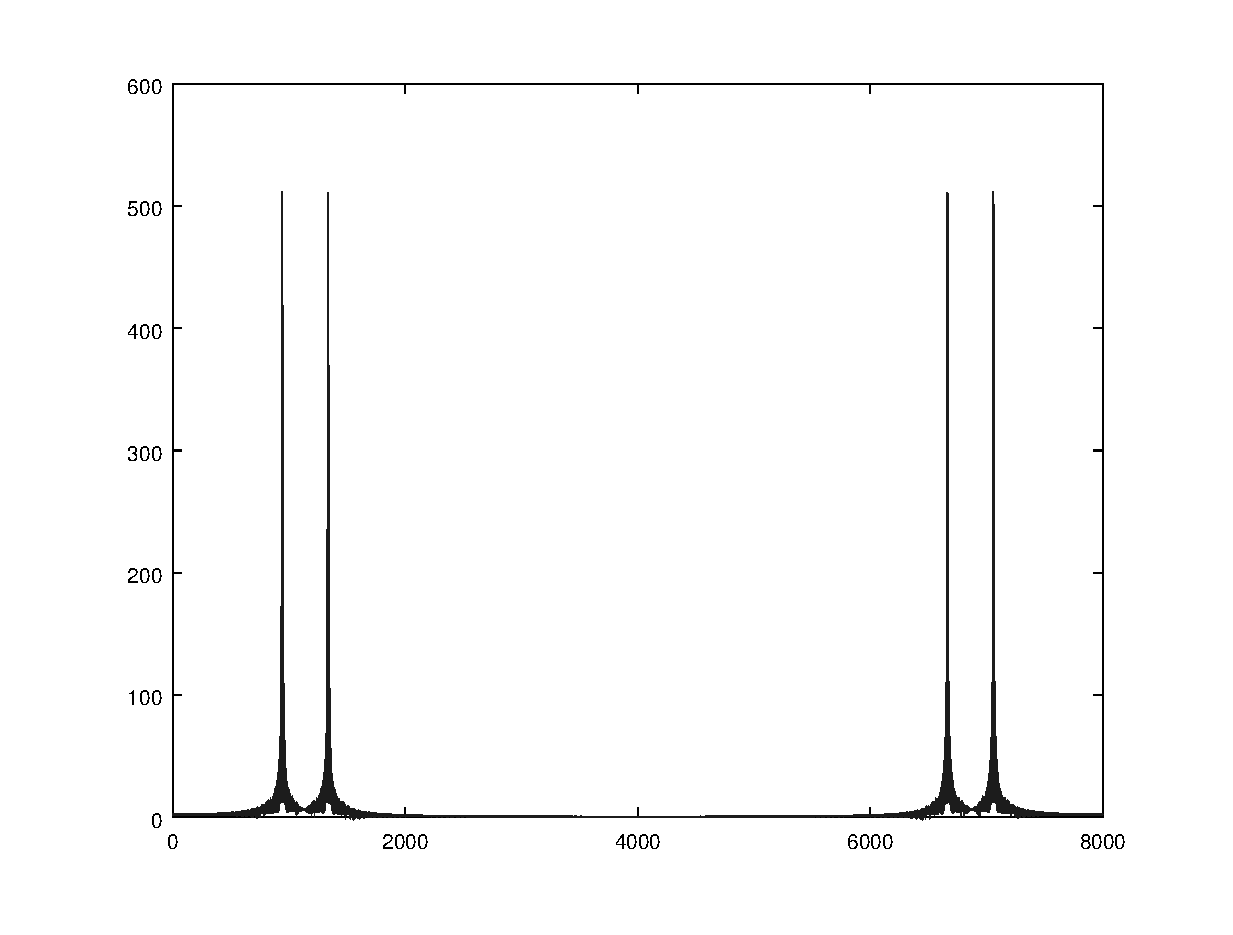
\includegraphics[scale=0.7]{moddft2.eps} 
\caption{Representació del mòdul de $X[k]$.}
\label{fig:moddft}
\end{figure}

La freqüència digital corresponent a cada índex $k$ de la DFT és $\frac{2\pi}{8000}k$, $k=0,1,\ldots, 7999$. Les freqüències digitals corresponents als pics són, doncs, $\frac{941}{4000}\pi$, $\frac{167}{500}\pi$, $\frac{833}{500}\pi$, $\frac{7059}{4000}\pi$. Com que estem treballant amb freqüències digitals, les dues últimes es podrien canviar per $-\frac{167}{500}\pi$ i $-\frac{941}{4000}\pi$.
\\

Recordem que la relació entre la freqüència digital i la freqüència analògica és $\Omega=\omega T$, on $\Omega$ és la freqüència digital, $\omega$ la freqüència analògica i $T$ el període de mostreig.
\\

Així doncs, les freqüències analògiques són $f_1=\frac{\omega_1}{2\pi T}=941\, Hz$  i $f_2=\frac{\omega_2}{2\pi T}=1336\, Hz$.
\\

Observant la Figura 1 del guió de la pràctica, la tecla pulsada és el zero.
\\

Tenint en compte la qüestió 2.6 i la linealitat de la DFT, $X[k]$ és gairebé la DFT d'un senyal discret de la forma:
$$
x[n] = A_1 \sin(2\pi\frac{941}{8000}n) + A_2 \sin(2\pi\frac{1336}{8000}n)
$$
(ho seria exactament si només tinguéssim els quatre pics), que és el senyal que s'obté mostrejant amb període $T=\frac{1}{8000}\,s$ ($x[n] = x(nT)$) un senyal analògic de la forma:
$$
x(t) = A_1 \sin(2\pi\, 941t) + A_2 \sin(2\pi\, 1336t)
$$
La petita distorsió que s'observa respecte el resultat esperat és deu probablement a l'existència de soroll i potser també a un petit desfasament.
\\

Les amplituds de la DFT als pics són $X[941] = 3,71-j511,46$, $X[1336] = 2,88-j511,33$, $X[6664] = 3,71+j511,46$ i $X[7059] = 3,71+j511,46$. En mòdul, les amplituds són $\overline{A_1}=511,48$ ($k=941,7059$) i $\overline{A_2}=511,34$ ($k=1336,6664$).
\\

Segons la qüestió 2.6, assumint que el senyal discret és exactament de la forma:
$$
x[n] = A_1 \sin(2\pi\frac{941}{8000}n) + A_2 \sin(2\pi\frac{1336}{8000}n),
$$
hauríem de tenir:
$$
\overline{A_1}=A_1\frac{8000}{2}=4000\,A_1,\quad \quad \overline{A_2}=A_2\frac{8000}{2}=4000\,A_2
$$

Amb els valors que hem obtingut per a $\overline{A_1}$ i $\overline{A_2}$, es té:
$$
A_1=\frac{\overline{A_1}}{4000}=0,12787,\quad\quad A_2=\frac{\overline{A_2}}{4000}=0,12784
$$
és a dir, $\overline{A_1}\approx\overline{A_2}\approx0,128$. 
\end{document}